\begin{subfigure}[b]{0.975\textwidth}
	%%%%%%%%%%%%%%%%%%%%%%%%%%%%%%%%%%%%%%%%%%%%%%%%%%%%%%%%%%%%%%%%%%%%%%%%%%%%
	% FH
	%%%%%%%%%%%%%%%%%%%%%%%%%%%%%%%%%%%%%%%%%%%%%%%%%%%%%%%%%%%%%%%%%%%%%%%%%%%%
	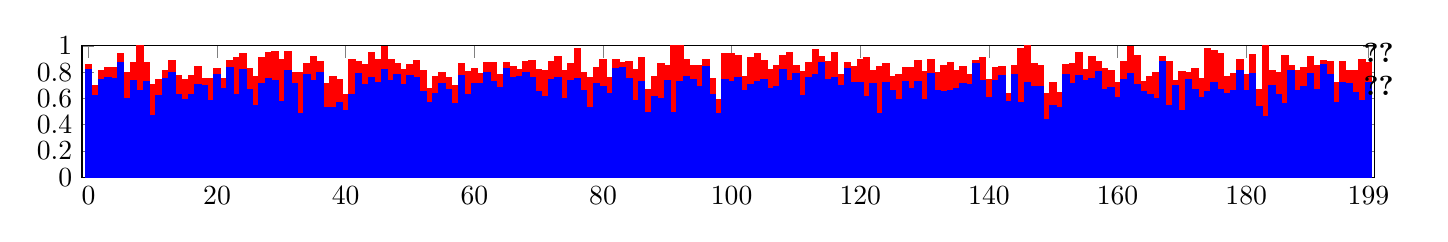
\begin{tikzpicture}
	    \begin{axis}[ybar stacked,
	    		   bar width=1,
	    		   enlarge x limits=0.005,
	            width=18cm,
	            height=3.25cm,
	            xmin=0,
	            xmax=199,
	            ymin=0,ymax=1,
	            ylabel=\begin{tabular}{l}\ref{plot:appendix-std-fh-rec} \Rec\\\ref{plot:appendix-std-fh-ue_np} \UE\end{tabular},
				y label style={
		        		rotate=270,
		        		at={(1.035, 0.8)}
		        },
		        xtick={0,20,40,60,80,100,120,140,160,180,199}]

	        % FH %%%%%%%%%%%%%%%%%%%%%%%%%%%%%%%%%%%%%%%%%%%%%%%%%%%%%%%%%%%
	        \addplot[ybar,blue,fill=blue] coordinates{
	            (0,0.820576)
				(1,0.620935)
				(2,0.745459)
				(3,0.756501)
				(4,0.749715)
				(5,0.875433)
				(6,0.599307)
				(7,0.73633)
				(8,0.657343)
				(9,0.726672)
				(10,0.469469)
				(11,0.618518)
				(12,0.751126)
				(13,0.795514)
				(14,0.626725)
				(15,0.588379)
				(16,0.628921)
				(17,0.706743)
				(18,0.694595)
				(19,0.582933)
				(20,0.78269)
				(21,0.677531)
				(22,0.837617)
				(23,0.628793)
				(24,0.818745)
				(25,0.664327)
				(26,0.542004)
				(27,0.715041)
				(28,0.748362)
				(29,0.737603)
				(30,0.578894)
				(31,0.810322)
				(32,0.716516)
				(33,0.480769)
				(34,0.780794)
				(35,0.73571)
				(36,0.794859)
				(37,0.526325)
				(38,0.53124)
				(39,0.567541)
				(40,0.507766)
				(41,0.630533)
				(42,0.790851)
				(43,0.703048)
				(44,0.757369)
				(45,0.718786)
				(46,0.820894)
				(47,0.735921)
				(48,0.778387)
				(49,0.703481)
				(50,0.775061)
				(51,0.760719)
				(52,0.654449)
				(53,0.569471)
				(54,0.634298)
				(55,0.716508)
				(56,0.668294)
				(57,0.562933)
				(58,0.771113)
				(59,0.627828)
				(60,0.716226)
				(61,0.715571)
				(62,0.798696)
				(63,0.727083)
				(64,0.680873)
				(65,0.825559)
				(66,0.759144)
				(67,0.766349)
				(68,0.793718)
				(69,0.757646)
				(70,0.652516)
				(71,0.617148)
				(72,0.745189)
				(73,0.758388)
				(74,0.597694)
				(75,0.733911)
				(76,0.747423)
				(77,0.659248)
				(78,0.528238)
				(79,0.715223)
				(80,0.687546)
				(81,0.639297)
				(82,0.826954)
				(83,0.834536)
				(84,0.74955)
				(85,0.583187)
				(86,0.725586)
				(87,0.492821)
				(88,0.614414)
				(89,0.598369)
				(90,0.732302)
				(91,0.494696)
				(92,0.729682)
				(93,0.763063)
				(94,0.744108)
				(95,0.6911)
				(96,0.841667)
				(97,0.631019)
				(98,0.487774)
				(99,0.744591)
				(100,0.725285)
				(101,0.759834)
				(102,0.659226)
				(103,0.705455)
				(104,0.730959)
				(105,0.743032)
				(106,0.671291)
				(107,0.693039)
				(108,0.817262)
				(109,0.735104)
				(110,0.790536)
				(111,0.618505)
				(112,0.75632)
				(113,0.779267)
				(114,0.874296)
				(115,0.744906)
				(116,0.75907)
				(117,0.696593)
				(118,0.82527)
				(119,0.720799)
				(120,0.717523)
				(121,0.613377)
				(122,0.714932)
				(123,0.484936)
				(124,0.722587)
				(125,0.65664)
				(126,0.593082)
				(127,0.724214)
				(128,0.672446)
				(129,0.724432)
				(130,0.594299)
				(131,0.790197)
				(132,0.656354)
				(133,0.648446)
				(134,0.656405)
				(135,0.67179)
				(136,0.711906)
				(137,0.702089)
				(138,0.868421)
				(139,0.735366)
				(140,0.607692)
				(141,0.734088)
				(142,0.774054)
				(143,0.577805)
				(144,0.782999)
				(145,0.565087)
				(146,0.718549)
				(147,0.691208)
				(148,0.692898)
				(149,0.440116)
				(150,0.546762)
				(151,0.526256)
				(152,0.779657)
				(153,0.710997)
				(154,0.774364)
				(155,0.738605)
				(156,0.75167)
				(157,0.801106)
				(158,0.669895)
				(159,0.686006)
				(160,0.606663)
				(161,0.741329)
				(162,0.790426)
				(163,0.707274)
				(164,0.653834)
				(165,0.628049)
				(166,0.600107)
				(167,0.879882)
				(168,0.543236)
				(169,0.701258)
				(170,0.50421)
				(171,0.741062)
				(172,0.668068)
				(173,0.608254)
				(174,0.651442)
				(175,0.72005)
				(176,0.670594)
				(177,0.638238)
				(178,0.656924)
				(179,0.808756)
				(180,0.660776)
				(181,0.785697)
				(182,0.540885)
				(183,0.460099)
				(184,0.697077)
				(185,0.629668)
				(186,0.563578)
				(187,0.812882)
				(188,0.661604)
				(189,0.689264)
				(190,0.785634)
				(191,0.666667)
				(192,0.854381)
				(193,0.781073)
				(194,0.566363)
				(195,0.720757)
				(196,0.713175)
				(197,0.646204)
				(198,0.585624)
				(199,0.717404)
			};
			\label{plot:appendix-std-fh-rec}

			% FH %%%%%%%%%%%%%%%%%%%%%%%%%%%%%%%%%%%%%%%%%%%%%%%%%%%%%%%%%%%
	        \addplot[ybar,red,fill=red] coordinates{
	            	(0,0.0388339)
				(1,0.0801161)
				(2,0.0646757)
				(3,0.0814632)
				(4,0.0883803)
				(5,0.0637949)
				(6,0.193444)
				(7,0.138419)
				(8,0.38922)
				(9,0.144015)
				(10,0.233846)
				(11,0.127493)
				(12,0.0588727)
				(13,0.0894878)
				(14,0.150206)
				(15,0.158432)
				(16,0.146981)
				(17,0.133982)
				(18,0.0597665)
				(19,0.165873)
				(20,0.0428106)
				(21,0.076243)
				(22,0.0482639)
				(23,0.279959)
				(24,0.123412)
				(25,0.163561)
				(26,0.227201)
				(27,0.195944)
				(28,0.203418)
				(29,0.221903)
				(30,0.313133)
				(31,0.146897)
				(32,0.0791316)
				(33,0.317051)
				(34,0.0875448)
				(35,0.17972)
				(36,0.0845785)
				(37,0.188723)
				(38,0.23176)
				(39,0.175005)
				(40,0.12123)
				(41,0.261734)
				(42,0.0900059)
				(43,0.152272)
				(44,0.188982)
				(45,0.178781)
				(46,0.174086)
				(47,0.158166)
				(48,0.0856406)
				(49,0.117156)
				(50,0.0850577)
				(51,0.128924)
				(52,0.154423)
				(53,0.102396)
				(54,0.133898)
				(55,0.0810617)
				(56,0.0887041)
				(57,0.133807)
				(58,0.0956535)
				(59,0.179468)
				(60,0.112156)
				(61,0.070576)
				(62,0.0704205)
				(63,0.147486)
				(64,0.10349)
				(65,0.0444816)
				(66,0.0846691)
				(67,0.0515929)
				(68,0.0862948)
				(69,0.129067)
				(70,0.168457)
				(71,0.193308)
				(72,0.138665)
				(73,0.15678)
				(74,0.215199)
				(75,0.133859)
				(76,0.233716)
				(77,0.139099)
				(78,0.229105)
				(79,0.118082)
				(80,0.208023)
				(81,0.118885)
				(82,0.0715021)
				(83,0.0379402)
				(84,0.132013)
				(85,0.238509)
				(86,0.18189)
				(87,0.176268)
				(88,0.15099)
				(89,0.270063)
				(90,0.116877)
				(91,0.526124)
				(92,0.465968)
				(93,0.128639)
				(94,0.10645)
				(95,0.157635)
				(96,0.0537497)
				(97,0.123581)
				(98,0.104248)
				(99,0.197499)
				(100,0.216158)
				(101,0.163542)
				(102,0.104896)
				(103,0.202421)
				(104,0.21075)
				(105,0.145433)
				(106,0.144669)
				(107,0.158535)
				(108,0.110919)
				(109,0.212777)
				(110,0.0602587)
				(111,0.185258)
				(112,0.11757)
				(113,0.191883)
				(114,0.0407769)
				(115,0.131618)
				(116,0.187032)
				(117,0.0849088)
				(118,0.0491253)
				(119,0.12066)
				(120,0.174843)
				(121,0.293742)
				(122,0.0968128)
				(123,0.358787)
				(124,0.139649)
				(125,0.11077)
				(126,0.184668)
				(127,0.110109)
				(128,0.16371)
				(129,0.164183)
				(130,0.207253)
				(131,0.10305)
				(132,0.139507)
				(133,0.199571)
				(134,0.213366)
				(135,0.142816)
				(136,0.130763)
				(137,0.0799865)
				(138,0.0208289)
				(139,0.17665)
				(140,0.135498)
				(141,0.103879)
				(142,0.0671498)
				(143,0.0552069)
				(144,0.0634646)
				(145,0.415923)
				(146,0.295095)
				(147,0.172013)
				(148,0.156288)
				(149,0.196799)
				(150,0.171709)
				(151,0.121521)
				(152,0.0764244)
				(153,0.150543)
				(154,0.17632)
				(155,0.0821303)
				(156,0.170161)
				(157,0.0824217)
				(158,0.15792)
				(159,0.123017)
				(160,0.115388)
				(161,0.138393)
				(162,0.205847)
				(163,0.219752)
				(164,0.0776161)
				(165,0.141217)
				(166,0.199196)
				(167,0.0377459)
				(168,0.340406)
				(169,0.0340024)
				(170,0.296313)
				(171,0.0533546)
				(172,0.157596)
				(173,0.141275)
				(174,0.326442)
				(175,0.244467)
				(176,0.273262)
				(177,0.124669)
				(178,0.131541)
				(179,0.0900059)
				(180,0.122966)
				(181,0.146845)
				(182,0.128665)
				(183,0.628558)
				(184,0.116852)
				(185,0.16735)
				(186,0.362796)
				(187,0.0365801)
				(188,0.152292)
				(189,0.144656)
				(190,0.135057)
				(191,0.184183)
				(192,0.0298444)
				(193,0.0957636)
				(194,0.156184)
				(195,0.160213)
				(196,0.100751)
				(197,0.163885)
				(198,0.312109)
				(199,0.151968)
			};
			\label{plot:appendix-std-fh-ue_np}

			% FH %%%%%%%%%%%%%%%%%%%%%%%%%%%%%%%%%%%%%%%%%%%%%%%%%%%%%%%%%%%
%	        \addplot[ybar,black,bar width=1,fill=black] coordinates{
%	            	(0,0.852501)
%				(1,0.689542)
%				(2,0.838582)
%				(3,0.837632)
%				(4,0.761383)
%				(5,0.68393)
%				(6,0.603564)
%				(7,0.779561)
%				(8,0.710871)
%				(9,0.8404)
%				(10,0.533869)
%				(11,0.819384)
%				(12,0.55658)
%				(13,0.880474)
%				(14,0.705926)
%				(15,0.709938)
%				(16,0.571654)
%				(17,0.758669)
%				(18,0.454461)
%				(19,0.647543)
%				(20,0.620945)
%				(21,0.541623)
%				(22,0.732336)
%				(23,0.737431)
%				(24,0.861817)
%				(25,0.707934)
%				(26,0.714057)
%				(27,0.797056)
%				(28,0.915093)
%				(29,0.766957)
%				(30,0.784056)
%				(31,0.872677)
%				(32,0.668261)
%				(33,0.567486)
%				(34,0.69128)
%				(35,0.607004)
%				(36,0.738686)
%				(37,0.887324)
%				(38,0.78507)
%				(39,0.803178)
%				(40,0.625138)
%				(41,0.69782)
%				(42,0.810493)
%				(43,0.77855)
%				(44,0.767272)
%				(45,0.80354)
%				(46,0.794694)
%				(47,0.865189)
%				(48,0.842397)
%				(49,0.761657)
%				(50,0.731411)
%				(51,0.841282)
%				(52,0.881744)
%				(53,0.52484)
%				(54,0.804032)
%				(55,0.763023)
%				(56,0.671953)
%				(57,0.460915)
%				(58,0.64313)
%				(59,0.855746)
%				(60,0.706046)
%				(61,0.679969)
%				(62,0.844521)
%				(63,0.877204)
%				(64,0.551853)
%				(65,0.774677)
%				(66,0.871948)
%				(67,0.781516)
%				(68,0.852344)
%				(69,0.753115)
%				(70,0.555924)
%				(71,0.450615)
%				(72,0.816744)
%				(73,0.840739)
%				(74,0.84152)
%				(75,0.932794)
%				(76,0.711466)
%				(77,0.744942)
%				(78,0.651381)
%				(79,0.783345)
%				(80,0.503406)
%				(81,0.864014)
%				(82,0.846275)
%				(83,0.879716)
%				(84,0.859932)
%				(85,0.639121)
%				(86,0.847517)
%				(87,0.888167)
%				(88,0.751177)
%				(89,0.427152)
%				(90,0.522087)
%				(91,0.455518)
%				(92,0.690407)
%				(93,0.679433)
%				(94,0.687025)
%				(95,0.860051)
%				(96,0.816653)
%				(97,0.764432)
%				(98,0.518118)
%				(99,0.551746)
%				(100,0.726513)
%				(101,0.819221)
%				(102,0.870047)
%				(103,0.654019)
%				(104,0.74708)
%				(105,0.78397)
%				(106,0.637064)
%				(107,0.737712)
%				(108,0.802078)
%				(109,0.924738)
%				(110,0.713512)
%				(111,0.786084)
%				(112,0.757133)
%				(113,0.86186)
%				(114,0.70789)
%				(115,0.909138)
%				(116,0.772135)
%				(117,0.810549)
%				(118,0.900358)
%				(119,0.804027)
%				(120,0.84925)
%				(121,0.824373)
%				(122,0.782986)
%				(123,0.350576)
%				(124,0.760363)
%				(125,0.839743)
%				(126,0.926822)
%				(127,0.791387)
%				(128,0.805002)
%				(129,0.681543)
%				(130,0.594578)
%				(131,0.761315)
%				(132,0.722273)
%				(133,0.871321)
%				(134,0.44164)
%				(135,0.819888)
%				(136,0.824018)
%				(137,0.866572)
%				(138,0.886959)
%				(139,0.841012)
%				(140,0.369569)
%				(141,0.743002)
%				(142,0.862358)
%				(143,0.848155)
%				(144,0.90221)
%				(145,0.648433)
%				(146,0.837022)
%				(147,0.882591)
%				(148,0.551568)
%				(149,0.891949)
%				(150,0.430412)
%				(151,0.595172)
%				(152,0.905244)
%				(153,0.766549)
%				(154,0.855644)
%				(155,0.838301)
%				(156,0.827014)
%				(157,0.765743)
%				(158,0.808694)
%				(159,0.847007)
%				(160,0.771344)
%				(161,0.850792)
%				(162,0.825784)
%				(163,0.901529)
%				(164,0.851683)
%				(165,0.829802)
%				(166,0.69114)
%				(167,0.738132)
%				(168,0.346829)
%				(169,0.871803)
%				(170,0.483953)
%				(171,0.696859)
%				(172,0.86368)
%				(173,0.6582)
%				(174,0.820501)
%				(175,0.825938)
%				(176,0.865552)
%				(177,0.820033)
%				(178,0.863282)
%				(179,0.866536)
%				(180,0.790604)
%				(181,0.55694)
%				(182,0.478259)
%				(183,0.544736)
%				(184,0.713715)
%				(185,0.593135)
%				(186,0.784906)
%				(187,0.725865)
%				(188,0.708254)
%				(189,0.654185)
%				(190,0.711117)
%				(191,0.64715)
%				(192,0.928658)
%				(193,0.788429)
%				(194,0.753231)
%				(195,0.802397)
%				(196,0.663364)
%				(197,0.841732)
%				(198,0.412347)
%				(199,0.623215)
%			};
			\label{plot:appendix-std-fh-ev}
		\end{axis}
	\end{tikzpicture}
\end{subfigure}
\begin{subfigure}[b]{0.975\textwidth}
	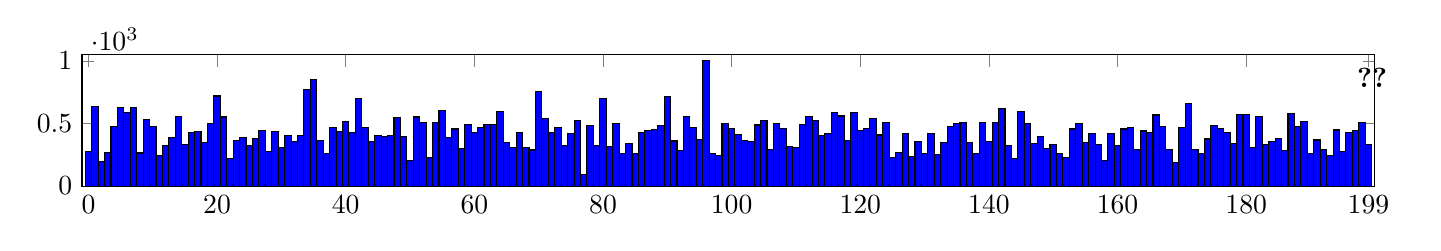
\begin{tikzpicture}
		\begin{axis}[ybar stacked,
				bar width=1,
				enlarge x limits=0.005,
	            width=18cm,
	            height=3.25cm,
	            xmin=0,
	            xmax=199,
	            ymin=0,ymax=1050,
	            ylabel=\begin{tabular}{l}\ref{plot:appendix-std-fh-sp} \K\end{tabular},
				y label style={
		        		rotate=270,
		        		at={(1.03, 0.8)}
		        },
		        scaled y ticks={base 10:-3},
		        xtick={0,20,40,60,80,100,120,140,160,180,199}]

			% FH SP %%%%%%%%%%%%%%%%%%%%%%%%%%%%%%%%%%%%%%%%%%%%%%%%%%%%%%%%
			\addplot[ybar,fill=blue] coordinates{
	        		(0,277)
				(1,637)
				(2,194)
				(3,271)
				(4,475)
				(5,629)
				(6,588)
				(7,630)
				(8,264)
				(9,532)
				(10,477)
				(11,245)
				(12,326)
				(13,387)
				(14,555)
				(15,335)
				(16,430)
				(17,438)
				(18,348)
				(19,502)
				(20,720)
				(21,552)
				(22,218)
				(23,361)
				(24,385)
				(25,325)
				(26,383)
				(27,444)
				(28,275)
				(29,434)
				(30,305)
				(31,404)
				(32,357)
				(33,401)
				(34,774)
				(35,851)
				(36,362)
				(37,263)
				(38,466)
				(39,434)
				(40,514)
				(41,425)
				(42,701)
				(43,468)
				(44,357)
				(45,402)
				(46,395)
				(47,407)
				(48,550)
				(49,394)
				(50,205)
				(51,552)
				(52,505)
				(53,226)
				(54,505)
				(55,606)
				(56,390)
				(57,456)
				(58,298)
				(59,489)
				(60,429)
				(61,469)
				(62,489)
				(63,493)
				(64,595)
				(65,347)
				(66,305)
				(67,427)
				(68,310)
				(69,288)
				(70,757)
				(71,542)
				(72,431)
				(73,471)
				(74,325)
				(75,419)
				(76,525)
				(77,89)
				(78,482)
				(79,327)
				(80,703)
				(81,318)
				(82,497)
				(83,258)
				(84,340)
				(85,257)
				(86,425)
				(87,445)
				(88,451)
				(89,485)
				(90,713)
				(91,360)
				(92,285)
				(93,558)
				(94,465)
				(95,369)
				(96,1007)
				(97,260)
				(98,245)
				(99,502)
				(100,457)
				(101,413)
				(102,367)
				(103,357)
				(104,488)
				(105,522)
				(106,290)
				(107,502)
				(108,460)
				(109,316)
				(110,309)
				(111,492)
				(112,553)
				(113,526)
				(114,407)
				(115,423)
				(116,587)
				(117,560)
				(118,365)
				(119,589)
				(120,442)
				(121,461)
				(122,539)
				(123,408)
				(124,509)
				(125,227)
				(126,270)
				(127,420)
				(128,236)
				(129,359)
				(130,261)
				(131,420)
				(132,254)
				(133,350)
				(134,477)
				(135,503)
				(136,510)
				(137,349)
				(138,259)
				(139,511)
				(140,357)
				(141,511)
				(142,617)
				(143,325)
				(144,222)
				(145,594)
				(146,503)
				(147,337)
				(148,394)
				(149,303)
				(150,335)
				(151,262)
				(152,231)
				(153,456)
				(154,501)
				(155,351)
				(156,421)
				(157,329)
				(158,206)
				(159,418)
				(160,324)
				(161,456)
				(162,470)
				(163,294)
				(164,440)
				(165,429)
				(166,568)
				(167,475)
				(168,294)
				(169,189)
				(170,466)
				(171,661)
				(172,293)
				(173,262)
				(174,376)
				(175,485)
				(176,463)
				(177,429)
				(178,337)
				(179,570)
				(180,570)
				(181,309)
				(182,555)
				(183,330)
				(184,356)
				(185,381)
				(186,281)
				(187,580)
				(188,473)
				(189,514)
				(190,260)
				(191,368)
				(192,295)
				(193,247)
				(194,448)
				(195,274)
				(196,431)
				(197,443)
				(198,509)
				(199,329)
			};
			\label{plot:appendix-std-fh-sp}

		\end{axis}
	\end{tikzpicture}
\end{subfigure}
\begin{subfigure}[b]{0.975\textwidth}
	%%%%%%%%%%%%%%%%%%%%%%%%%%%%%%%%%%%%%%%%%%%%%%%%%%%%%%%%%%%%%%%%%%%%%%%%%%%%
	% VC
	%%%%%%%%%%%%%%%%%%%%%%%%%%%%%%%%%%%%%%%%%%%%%%%%%%%%%%%%%%%%%%%%%%%%%%%%%%%%
	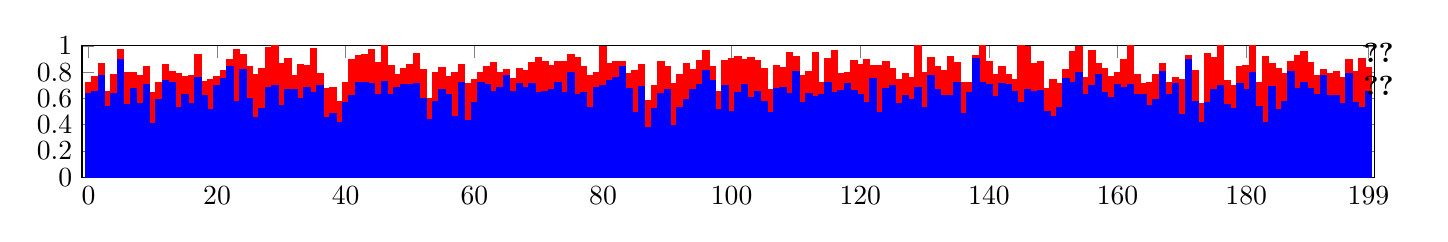
\begin{tikzpicture}
	    \begin{axis}[ybar stacked,
	    		   bar width=1,
	    		   enlarge x limits=0.005,
	            width=18cm,
	            height=3.25cm,
	            xmin=0,
	            xmax=199,
	            ymin=0,ymax=1,
	            ylabel=\begin{tabular}{l}\ref{plot:appendix-std-vc-rec} \Rec\\\ref{plot:appendix-std-vc-ue_np} \UE\end{tabular},
				y label style={
		        		rotate=270,
		        		at={(1.035, 0.8)}
		        },
		        xtick={0,20,40,60,80,100,120,140,160,180,199}]

	        % VC %%%%%%%%%%%%%%%%%%%%%%%%%%%%%%%%%%%%%%%%%%%%%%%%%%%%%%%%%%%
	        \addplot[ybar,blue,bar width=1,fill=blue] coordinates{
	            (0,0.638089)
				(1,0.64922)
				(2,0.776236)
				(3,0.533915)
				(4,0.639034)
				(5,0.898039)
				(6,0.552253)
				(7,0.678277)
				(8,0.562465)
				(9,0.705805)
				(10,0.409776)
				(11,0.590384)
				(12,0.739302)
				(13,0.71774)
				(14,0.529222)
				(15,0.627492)
				(16,0.563122)
				(17,0.761056)
				(18,0.620721)
				(19,0.513422)
				(20,0.701121)
				(21,0.751847)
				(22,0.843665)
				(23,0.574453)
				(24,0.819292)
				(25,0.601998)
				(26,0.454743)
				(27,0.522767)
				(28,0.679742)
				(29,0.696155)
				(30,0.543377)
				(31,0.664669)
				(32,0.666992)
				(33,0.595654)
				(34,0.683304)
				(35,0.644001)
				(36,0.700524)
				(37,0.451913)
				(38,0.481555)
				(39,0.416378)
				(40,0.567901)
				(41,0.618926)
				(42,0.723179)
				(43,0.723465)
				(44,0.715706)
				(45,0.629439)
				(46,0.729647)
				(47,0.631672)
				(48,0.682496)
				(49,0.708561)
				(50,0.7039)
				(51,0.714164)
				(52,0.594886)
				(53,0.438942)
				(54,0.577594)
				(55,0.670555)
				(56,0.629883)
				(57,0.458133)
				(58,0.72402)
				(59,0.434258)
				(60,0.569308)
				(61,0.719031)
				(62,0.708272)
				(63,0.653646)
				(64,0.679351)
				(65,0.77303)
				(66,0.649834)
				(67,0.713215)
				(68,0.685059)
				(69,0.715834)
				(70,0.641261)
				(71,0.654669)
				(72,0.663437)
				(73,0.719155)
				(74,0.645581)
				(75,0.792735)
				(76,0.62746)
				(77,0.643399)
				(78,0.529466)
				(79,0.680915)
				(80,0.701059)
				(81,0.737118)
				(82,0.75659)
				(83,0.838813)
				(84,0.671597)
				(85,0.492077)
				(86,0.687567)
				(87,0.380287)
				(88,0.524582)
				(89,0.639139)
				(90,0.66508)
				(91,0.389261)
				(92,0.526507)
				(93,0.587838)
				(94,0.669098)
				(95,0.706451)
				(96,0.812069)
				(97,0.738976)
				(98,0.511912)
				(99,0.698193)
				(100,0.50305)
				(101,0.643763)
				(102,0.706488)
				(103,0.603747)
				(104,0.651762)
				(105,0.574516)
				(106,0.488527)
				(107,0.678167)
				(108,0.679861)
				(109,0.634457)
				(110,0.807237)
				(111,0.565634)
				(112,0.635426)
				(113,0.61548)
				(114,0.631556)
				(115,0.720219)
				(116,0.640571)
				(117,0.660752)
				(118,0.715993)
				(119,0.656476)
				(120,0.63259)
				(121,0.565209)
				(122,0.751131)
				(123,0.490247)
				(124,0.674979)
				(125,0.700758)
				(126,0.559635)
				(127,0.621475)
				(128,0.588475)
				(129,0.681358)
				(130,0.528933)
				(131,0.773342)
				(132,0.667253)
				(133,0.618866)
				(134,0.618608)
				(135,0.723598)
				(136,0.486335)
				(137,0.645291)
				(138,0.903178)
				(139,0.718077)
				(140,0.708923)
				(141,0.617359)
				(142,0.714955)
				(143,0.702051)
				(144,0.651722)
				(145,0.566265)
				(146,0.663558)
				(147,0.649118)
				(148,0.662712)
				(149,0.498166)
				(150,0.459502)
				(151,0.531939)
				(152,0.747966)
				(153,0.722862)
				(154,0.799819)
				(155,0.632093)
				(156,0.697891)
				(157,0.782057)
				(158,0.64407)
				(159,0.605694)
				(160,0.706604)
				(161,0.683058)
				(162,0.702578)
				(163,0.631902)
				(164,0.625922)
				(165,0.542683)
				(166,0.592851)
				(167,0.803242)
				(168,0.627056)
				(169,0.71174)
				(170,0.473621)
				(171,0.89428)
				(172,0.578357)
				(173,0.41272)
				(174,0.570987)
				(175,0.664262)
				(176,0.70082)
				(177,0.555468)
				(178,0.520661)
				(179,0.71638)
				(180,0.6633)
				(181,0.797115)
				(182,0.541239)
				(183,0.41454)
				(184,0.689367)
				(185,0.518376)
				(186,0.575506)
				(187,0.803479)
				(188,0.673434)
				(189,0.720472)
				(190,0.676836)
				(191,0.631171)
				(192,0.770465)
				(193,0.61855)
				(194,0.61793)
				(195,0.556925)
				(196,0.78561)
				(197,0.567199)
				(198,0.528658)
				(199,0.653434)
			};
			\label{plot:appendix-std-vc-rec}

			% VC %%%%%%%%%%%%%%%%%%%%%%%%%%%%%%%%%%%%%%%%%%%%%%%%%%%%%%%%%%%
	        \addplot[ybar,red,bar width=1,fill=red] coordinates{
	            	(0,0.085116)
				(1,0.117784)
				(2,0.0870461)
				(3,0.117629)
				(4,0.139157)
				(5,0.076243)
				(6,0.241203)
				(7,0.117318)
				(8,0.212563)
				(9,0.139883)
				(10,0.231223)
				(11,0.127473)
				(12,0.117706)
				(13,0.0872922)
				(14,0.25891)
				(15,0.139934)
				(16,0.211281)
				(17,0.173062)
				(18,0.106256)
				(19,0.23301)
				(20,0.0658804)
				(21,0.0615929)
				(22,0.0483417)
				(23,0.395522)
				(24,0.11408)
				(25,0.236611)
				(26,0.32641)
				(27,0.306999)
				(28,0.306695)
				(29,0.335859)
				(30,0.320205)
				(31,0.241002)
				(32,0.107655)
				(33,0.264182)
				(34,0.167888)
				(35,0.334072)
				(36,0.0883803)
				(37,0.2213)
				(38,0.201683)
				(39,0.161774)
				(40,0.151126)
				(41,0.279221)
				(42,0.205394)
				(43,0.209111)
				(44,0.258677)
				(45,0.246643)
				(46,0.302381)
				(47,0.219202)
				(48,0.0957248)
				(49,0.116424)
				(50,0.150271)
				(51,0.225011)
				(52,0.226903)
				(53,0.160388)
				(54,0.221216)
				(55,0.161152)
				(56,0.139015)
				(57,0.335024)
				(58,0.134241)
				(59,0.276455)
				(60,0.175005)
				(61,0.0798181)
				(62,0.132434)
				(63,0.219629)
				(64,0.116074)
				(65,0.0476033)
				(66,0.100427)
				(67,0.113289)
				(68,0.12996)
				(69,0.159151)
				(70,0.272116)
				(71,0.229247)
				(72,0.188516)
				(73,0.162)
				(74,0.237498)
				(75,0.143283)
				(76,0.280361)
				(77,0.196372)
				(78,0.24529)
				(79,0.1193)
				(80,0.297038)
				(81,0.128497)
				(82,0.123743)
				(83,0.0442484)
				(84,0.120854)
				(85,0.317453)
				(86,0.171644)
				(87,0.205323)
				(88,0.171048)
				(89,0.242039)
				(90,0.174623)
				(91,0.326306)
				(92,0.251915)
				(93,0.277861)
				(94,0.14724)
				(95,0.184118)
				(96,0.153173)
				(97,0.101463)
				(98,0.138691)
				(99,0.191812)
				(100,0.403352)
				(101,0.274655)
				(102,0.189299)
				(103,0.307304)
				(104,0.236158)
				(105,0.254539)
				(106,0.177292)
				(107,0.174636)
				(108,0.155692)
				(109,0.317511)
				(110,0.10724)
				(111,0.205957)
				(112,0.168198)
				(113,0.336215)
				(114,0.0921626)
				(115,0.181896)
				(116,0.326228)
				(117,0.125802)
				(118,0.081515)
				(119,0.233612)
				(120,0.222699)
				(121,0.331067)
				(122,0.0949476)
				(123,0.360438)
				(124,0.202563)
				(125,0.122577)
				(126,0.185232)
				(127,0.167136)
				(128,0.166838)
				(129,0.387821)
				(130,0.266086)
				(131,0.13996)
				(132,0.174753)
				(133,0.195484)
				(134,0.303308)
				(135,0.149552)
				(136,0.230743)
				(137,0.0742094)
				(138,0.0192874)
				(139,0.292505)
				(140,0.172557)
				(141,0.161307)
				(142,0.130841)
				(143,0.0763596)
				(144,0.0880305)
				(145,0.495359)
				(146,0.334441)
				(147,0.214429)
				(148,0.219221)
				(149,0.17779)
				(150,0.285322)
				(151,0.182512)
				(152,0.0723182)
				(153,0.23198)
				(154,0.191786)
				(155,0.123341)
				(156,0.265439)
				(157,0.0807378)
				(158,0.18097)
				(159,0.157758)
				(160,0.0916574)
				(161,0.21483)
				(162,0.328236)
				(163,0.152305)
				(164,0.0881082)
				(165,0.178121)
				(166,0.188969)
				(167,0.0641835)
				(168,0.0942351)
				(169,0.0441189)
				(170,0.269538)
				(171,0.0344428)
				(172,0.235737)
				(173,0.147862)
				(174,0.367634)
				(175,0.249519)
				(176,0.384661)
				(177,0.179293)
				(178,0.17417)
				(179,0.124371)
				(180,0.18926)
				(181,0.21268)
				(182,0.175413)
				(183,0.503915)
				(184,0.173172)
				(185,0.307122)
				(186,0.215309)
				(187,0.0762171)
				(188,0.251449)
				(189,0.239377)
				(190,0.199086)
				(191,0.144028)
				(192,0.0499479)
				(193,0.173794)
				(194,0.188153)
				(195,0.198671)
				(196,0.106593)
				(197,0.233502)
				(198,0.374441)
				(199,0.181683)
			};
			\label{plot:appendix-std-vc-ue_np}

			% VC %%%%%%%%%%%%%%%%%%%%%%%%%%%%%%%%%%%%%%%%%%%%%%%%%%%%%%%%%%%
%	        \addplot[ybar,black,bar width=1,fill=black] coordinates{
%	            	(0,0.888332)
%				(1,0.697693)
%				(2,0.915603)
%				(3,0.814496)
%				(4,0.736682)
%				(5,0.699521)
%				(6,0.566906)
%				(7,0.731055)
%				(8,0.879734)
%				(9,0.848283)
%				(10,0.52021)
%				(11,0.881664)
%				(12,0.632098)
%				(13,0.897249)
%				(14,0.753958)
%				(15,0.801183)
%				(16,0.520096)
%				(17,0.762815)
%				(18,0.442492)
%				(19,0.529802)
%				(20,0.500144)
%				(21,0.478268)
%				(22,0.89274)
%				(23,0.744651)
%				(24,0.85462)
%				(25,0.704257)
%				(26,0.715799)
%				(27,0.788583)
%				(28,0.939)
%				(29,0.737894)
%				(30,0.850657)
%				(31,0.824001)
%				(32,0.704919)
%				(33,0.639717)
%				(34,0.628739)
%				(35,0.426339)
%				(36,0.70332)
%				(37,0.874743)
%				(38,0.816782)
%				(39,0.844469)
%				(40,0.657284)
%				(41,0.747674)
%				(42,0.769373)
%				(43,0.761309)
%				(44,0.734522)
%				(45,0.780661)
%				(46,0.743102)
%				(47,0.848109)
%				(48,0.834599)
%				(49,0.773265)
%				(50,0.887702)
%				(51,0.802843)
%				(52,0.880853)
%				(53,0.669669)
%				(54,0.788115)
%				(55,0.698981)
%				(56,0.58746)
%				(57,0.281075)
%				(58,0.671188)
%				(59,0.840537)
%				(60,0.722591)
%				(61,0.680708)
%				(62,0.863481)
%				(63,0.861621)
%				(64,0.498339)
%				(65,0.836295)
%				(66,0.927191)
%				(67,0.766393)
%				(68,0.860936)
%				(69,0.834856)
%				(70,0.486867)
%				(71,0.452426)
%				(72,0.787331)
%				(73,0.843607)
%				(74,0.889662)
%				(75,0.929392)
%				(76,0.569526)
%				(77,0.900535)
%				(78,0.627321)
%				(79,0.84963)
%				(80,0.442325)
%				(81,0.902516)
%				(82,0.862239)
%				(83,0.911682)
%				(84,0.836308)
%				(85,0.698891)
%				(86,0.794469)
%				(87,0.880006)
%				(88,0.685234)
%				(89,0.404046)
%				(90,0.381208)
%				(91,0.664327)
%				(92,0.624626)
%				(93,0.562404)
%				(94,0.621522)
%				(95,0.84502)
%				(96,0.76478)
%				(97,0.822346)
%				(98,0.447425)
%				(99,0.524686)
%				(100,0.668577)
%				(101,0.7337)
%				(102,0.866101)
%				(103,0.662233)
%				(104,0.768906)
%				(105,0.727214)
%				(106,0.618355)
%				(107,0.688478)
%				(108,0.773179)
%				(109,0.907545)
%				(110,0.785691)
%				(111,0.766541)
%				(112,0.752184)
%				(113,0.812822)
%				(114,0.54136)
%				(115,0.906689)
%				(116,0.686983)
%				(117,0.696806)
%				(118,0.916794)
%				(119,0.712813)
%				(120,0.822674)
%				(121,0.844595)
%				(122,0.747893)
%				(123,0.361931)
%				(124,0.731062)
%				(125,0.86553)
%				(126,0.949848)
%				(127,0.744306)
%				(128,0.746883)
%				(129,0.622466)
%				(130,0.615965)
%				(131,0.733576)
%				(132,0.822595)
%				(133,0.86488)
%				(134,0.406065)
%				(135,0.824197)
%				(136,0.812876)
%				(137,0.899146)
%				(138,0.924169)
%				(139,0.816725)
%				(140,0.393068)
%				(141,0.654129)
%				(142,0.865473)
%				(143,0.835687)
%				(144,0.890121)
%				(145,0.592695)
%				(146,0.778358)
%				(147,0.90806)
%				(148,0.57955)
%				(149,0.930214)
%				(150,0.531504)
%				(151,0.635694)
%				(152,0.920866)
%				(153,0.72211)
%				(154,0.868932)
%				(155,0.880689)
%				(156,0.742921)
%				(157,0.81561)
%				(158,0.840129)
%				(159,0.836695)
%				(160,0.832071)
%				(161,0.803883)
%				(162,0.797868)
%				(163,0.889264)
%				(164,0.890233)
%				(165,0.83068)
%				(166,0.68787)
%				(167,0.723988)
%				(168,0.535869)
%				(169,0.923853)
%				(170,0.463941)
%				(171,0.695641)
%				(172,0.870357)
%				(173,0.808502)
%				(174,0.840231)
%				(175,0.79066)
%				(176,0.857112)
%				(177,0.829086)
%				(178,0.894748)
%				(179,0.856097)
%				(180,0.734308)
%				(181,0.53212)
%				(182,0.556064)
%				(183,0.706824)
%				(184,0.721138)
%				(185,0.706306)
%				(186,0.79752)
%				(187,0.688736)
%				(188,0.653541)
%				(189,0.534808)
%				(190,0.72837)
%				(191,0.68952)
%				(192,0.943263)
%				(193,0.819918)
%				(194,0.752607)
%				(195,0.826472)
%				(196,0.678393)
%				(197,0.818696)
%				(198,0.394216)
%				(199,0.712391)
%			};
%			\label{plot:appendix-std-vc-ev}
		\end{axis}
	\end{tikzpicture}
\end{subfigure}
\begin{subfigure}[b]{0.975\textwidth}
	\hskip 8px
	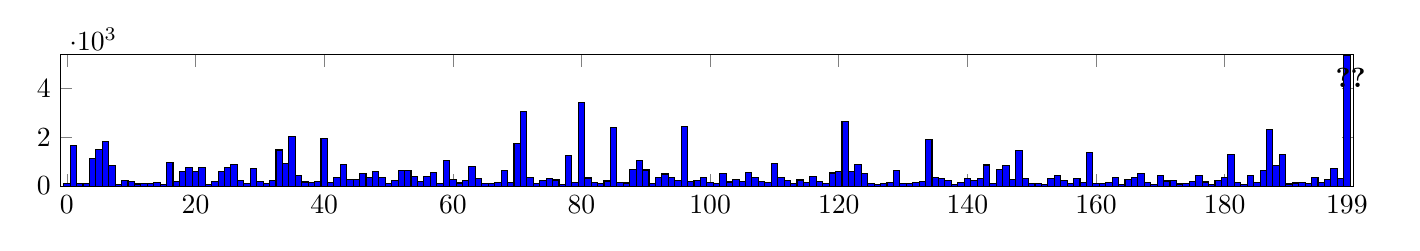
\begin{tikzpicture}
		\begin{axis}[ybar stacked,
				bar width=1,
				enlarge x limits=0.005,
	            width=18cm,
	            height=3.25cm,
	            xmin=0,
	            xmax=199,
	            ymin=0,ymax=5400,
	            ylabel=\begin{tabular}{l}\ref{plot:appendix-std-vc-sp} \K\end{tabular},
				y label style={
		        		rotate=270,
		        		at={(1.03, 0.8)}
		        },
		        scaled y ticks={base 10:-3},
		        xtick={0,20,40,60,80,100,120,140,160,180,199}]

			% VC SP %%%%%%%%%%%%%%%%%%%%%%%%%%%%%%%%%%%%%%%%%%%%%%%%%%%%%%%%
			\addplot[ybar,fill=blue] coordinates{
	        		(0,103)
				(1,1649)
				(2,87)
				(3,122)
				(4,1141)
				(5,1506)
				(6,1814)
				(7,827)
				(8,61)
				(9,224)
				(10,173)
				(11,83)
				(12,122)
				(13,100)
				(14,145)
				(15,74)
				(16,966)
				(17,186)
				(18,602)
				(19,753)
				(20,604)
				(21,763)
				(22,61)
				(23,198)
				(24,584)
				(25,777)
				(26,879)
				(27,245)
				(28,115)
				(29,725)
				(30,172)
				(31,106)
				(32,236)
				(33,1482)
				(34,924)
				(35,2041)
				(36,428)
				(37,165)
				(38,140)
				(39,174)
				(40,1959)
				(41,151)
				(42,342)
				(43,880)
				(44,280)
				(45,255)
				(46,509)
				(47,358)
				(48,583)
				(49,345)
				(50,92)
				(51,235)
				(52,631)
				(53,652)
				(54,390)
				(55,189)
				(56,408)
				(57,574)
				(58,123)
				(59,1034)
				(60,274)
				(61,124)
				(62,233)
				(63,791)
				(64,297)
				(65,120)
				(66,120)
				(67,139)
				(68,640)
				(69,131)
				(70,1749)
				(71,3066)
				(72,352)
				(73,97)
				(74,223)
				(75,307)
				(76,251)
				(77,78)
				(78,1242)
				(79,149)
				(80,3423)
				(81,331)
				(82,152)
				(83,109)
				(84,207)
				(85,2418)
				(86,138)
				(87,126)
				(88,679)
				(89,1033)
				(90,660)
				(91,96)
				(92,362)
				(93,496)
				(94,348)
				(95,235)
				(96,2446)
				(97,173)
				(98,217)
				(99,347)
				(100,151)
				(101,91)
				(102,512)
				(103,165)
				(104,261)
				(105,171)
				(106,559)
				(107,366)
				(108,194)
				(109,151)
				(110,925)
				(111,363)
				(112,236)
				(113,100)
				(114,248)
				(115,152)
				(116,375)
				(117,199)
				(118,105)
				(119,536)
				(120,592)
				(121,2652)
				(122,601)
				(123,869)
				(124,528)
				(125,107)
				(126,58)
				(127,93)
				(128,135)
				(129,634)
				(130,94)
				(131,108)
				(132,147)
				(133,187)
				(134,1931)
				(135,340)
				(136,315)
				(137,245)
				(138,58)
				(139,151)
				(140,322)
				(141,241)
				(142,297)
				(143,867)
				(144,96)
				(145,678)
				(146,843)
				(147,271)
				(148,1466)
				(149,321)
				(150,100)
				(151,121)
				(152,72)
				(153,329)
				(154,431)
				(155,215)
				(156,90)
				(157,299)
				(158,135)
				(159,1395)
				(160,99)
				(161,115)
				(162,152)
				(163,348)
				(164,77)
				(165,258)
				(166,344)
				(167,527)
				(168,161)
				(169,54)
				(170,443)
				(171,210)
				(172,229)
				(173,85)
				(174,98)
				(175,184)
				(176,452)
				(177,169)
				(178,70)
				(179,245)
				(180,352)
				(181,1293)
				(182,155)
				(183,72)
				(184,418)
				(185,140)
				(186,626)
				(187,2343)
				(188,829)
				(189,1306)
				(190,86)
				(191,127)
				(192,131)
				(193,99)
				(194,370)
				(195,140)
				(196,265)
				(197,707)
				(198,297)
				(199,5386)
			};
			\label{plot:appendix-std-vc-sp}

		\end{axis}
	\end{tikzpicture}
\end{subfigure}
